\documentclass{article}
\usepackage{graphicx}
\usepackage{amsmath}
\usepackage[margin=2.5cm]{geometry}
\usepackage{hyperref}
\usepackage{booktabs}
\usepackage{placeins}

\begin{document}
\title{Kernels and Random Feature Maps}
\author{Ludovico Passoni}
\date{\today}
\maketitle
\begin{center}
\subsection*{Declaration of Originality}

I declare that this material, which I now submit for assessment, is entirely my own work and
has not been taken from the work of others, save and to the extent that such work has been
cited and acknowledged within the text of my work. I understand that plagiarism, collusion,
and copying are grave and serious offences in the university and accept the penalties that
would be imposed should I engage in plagiarism, collusion or copying. This assignment, or
any part of it, has not been previously submitted by me or any other person for assessment
on this or any other course of study.
\end{center}
\section{Introduction}

Linear models are simple to optimize and to interpret, but their expressiveness is inherently limited: when the data is not separable by a linear boundary, no choice of parameters can solve the problem. Kernel methods overcome this limitation by implicitly mapping the data into a much higher-dimensional (potentially infinite-dimensional) feature space, allowing a linear classifier to operate in this new space without ever computing its coordinates explicitly. A more recent alternative, Random Fourier Features, approximates the same kernel through an explicit, finite-dimensional feature map, reducing the problem back to a simple linear model over transformed features.

In this project, three approaches are implemented from scratch and compared: a linear SVM trained via subgradient descent, a kernel SVM with an RBF kernel trained via Sequential Minimal Optimization (SMO), and a linear model trained on top of Random Fourier Features. The comparison is carried out on a synthetic dataset designed to be non-linearly separable by construction (a XOR pattern) and on a real-world dataset (parity classification on handwritten digits), with the goal of empirically showing the limitations of the linear model, the advantage of the kernel trick, and the ability of random features to approximate the performance of the exact kernel at a lower computational cost.

The rest of the report is organized as follows: Section 2 describes the methodology (datasets and implemented models), Section 3 presents the experimental results and the extensions explored, Section 4 critically discusses the results obtained, and Section 5 concludes the work.
\section{Methodology}

\subsection{Datasets}

The choice of datasets is motivated by the goal of highlighting the difficulties that a linear model encounters in certain settings, and how kernel-based methods instead achieve substantially better results. In both cases, the same criterion guided the choice: constructing (or selecting) a problem in which non-linear separation is actually necessary, avoiding datasets where a simple linear model would already be sufficient to obtain good performance.

For the synthetic dataset, an XOR pattern was chosen: 400 total points, evenly split into four clusters sampled from Gaussian distributions, centered in the four quadrants of the Cartesian plane (at distance $c=1.5$ from the origin along each axis). Labels are assigned based on the quadrant of membership, following the classic XOR scheme: the two quadrants on the same diagonal (where the coordinates share the same sign) share one label, while the other two share the opposite label. This makes the dataset non-linearly separable by construction: no straight line can correctly divide the two classes, regardless of how the linear model's parameters are chosen. The standard deviation of the clusters ($\text{std}=0.6$) was chosen as a trade-off: a value too low would make the four clusters perfectly separated, oversimplifying the problem even for a linear model near the boundaries; a value too high would cause excessive overlap between clusters, making the problem hard even for kernel methods. Figure~\ref{fig:xor_dataset} shows the resulting distribution.

\begin{figure}[h]
    \centering
    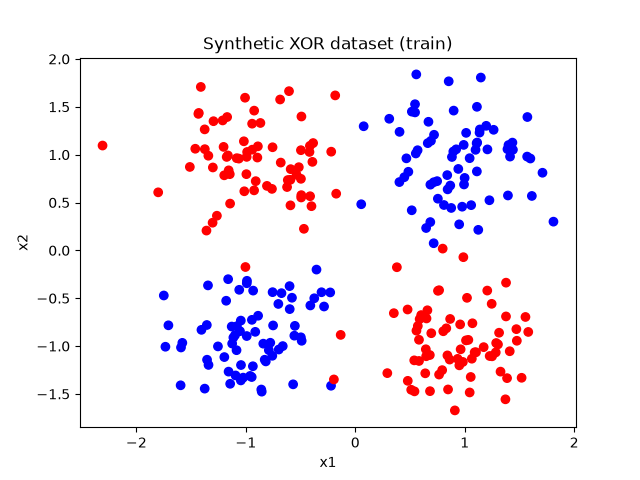
\includegraphics[width=0.6\textwidth]{../plots/xor_dataset.png}
    \caption{Synthetic XOR dataset (training set), colored by class label.}
    \label{fig:xor_dataset}
\end{figure}

For the real-world dataset, \texttt{sklearn.datasets.load\_digits()} was chosen, a dataset of 1797 grayscale $8\times 8$ images of handwritten digits (0-9), here used by flattening each image into a 64-feature vector. A natural comparison would have been classifying a single pair of digits (e.g., ``3'' vs ``8''). This option was discarded because, with only a few hundred samples in a 64-dimensional space, problems of this kind tend to be almost perfectly separable even by a linear model, making the comparison with kernel methods largely uninformative. The ``even vs. odd'' task (digits 0,2,4,6,8 against 1,3,5,7,9) was therefore chosen instead, as it groups visually heterogeneous shapes within the same class (e.g., ``0'' and ``8'' do not resemble each other at all, despite sharing the same label), producing a genuinely non-linear decision boundary.

\subsubsection{Linear SVM}

The linear SVM in the non-separable case is obtained by minimizing
\begin{equation}
    F(\mathbf{w}) = \frac{1}{m}\sum_{t=1}^m \ell^H_t(\mathbf{w}) + \frac{\lambda}{2}\|\mathbf{w}\|^2
\end{equation}
where $\ell^H_t(\mathbf{w}) = \left[1 - y_t\, \mathbf{w}^\top\mathbf{x}_t\right]_+$ is the hinge loss of the $t$-th example and $\lambda > 0$ is the regularization parameter. To include a bias term without introducing a separate, unregularized parameter, the homogeneous coordinates trick is used: every point $\mathbf{x}$ is extended with a constant component equal to 1, $\mathbf{x}' = (\mathbf{x}, 1)$, so that $\mathbf{w}'^\top\mathbf{x}' = \mathbf{w}^\top\mathbf{x} + b$ for a weight vector extended by one dimension, whose last component acts as the bias and is regularized along with the rest.

The model is trained with the Pegasos algorithm: at each iteration $t$, an example is drawn at random and a subgradient descent step is performed on $\ell_t(\mathbf{w}) = \ell^H_t(\mathbf{w}) + \frac{\lambda}{2}\|\mathbf{w}\|^2$, which is strongly convex, with a decreasing learning rate $\eta_t = 1/(\lambda t)$. This model is used both as the baseline on the raw features, and, unchanged, as the linear classifier trained on top of Random Fourier Features (Section~\ref{sssec:rff}).

\subsubsection{Kernel SVM (RBF, via SMO)}

When the training set is not linearly separable, the minimizer $\mathbf{w}^*$ of $F$ can still be written as a linear combination of the training points weighted by their labels, $\mathbf{w}^* = \sum_t \alpha_t y_t \mathbf{x}_t$. This result is what makes the kernel trick applicable: by replacing the inner product $\mathbf{x}^\top\mathbf{x}'$ with a kernel function $K(\mathbf{x}, \mathbf{x}')$, the SVM can implicitly operate in a high- (or infinite-) dimensional feature space $\mathcal{H}_K$, known as a Reproducing Kernel Hilbert Space (RKHS), without ever explicitly computing its coordinates.

A symmetric function $K$ is a valid kernel if and only if, for any finite set of points, the matrix $K$ with entries $K_{ij} = K(\mathbf{x}_i, \mathbf{x}_j)$ is positive semidefinite. The Gaussian (or RBF) kernel satisfies this condition and is, moreover, universal: for every continuous function $f$ and every $\epsilon>0$, there exists a finite combination of Gaussian kernels centered at suitable points that approximates $f$ to within $\epsilon$. This theoretically justifies the use of the Gaussian kernel in this assignment: a Gaussian kernel SVM can, in principle, approximate any continuous decision boundary, including the synthetic dataset's XOR pattern. The kernel function used is $K(\mathbf{x}, \mathbf{x}') = \exp(-\gamma\|\mathbf{x}-\mathbf{x}'\|^2)$, and the resulting decision function is $f(\mathbf{x}) = \sum_i \alpha_i y_i K(\mathbf{x}_i, \mathbf{x}) + b$.

The dual problem that determines the $\alpha_i$ is solved with the Sequential Minimal Optimization (SMO) algorithm: at each step, two multipliers $\alpha_i, \alpha_j$ are jointly updated in closed form, keeping all others fixed, until convergence. The bandwidth $\gamma$ is set using the median heuristic, $\gamma = 1/(2\hat\sigma^2)$, where $\hat\sigma$ is the median pairwise Euclidean distance between training points (Section~\ref{ssec:gamma_ext}).

\subsubsection{Random Fourier Features + Linear Model}
\label{sssec:rff}

The universal but implicit nature of the Gaussian kernel (an infinite-dimensional RKHS) is precisely what Random Fourier Features aim to make explicit and finite-dimensional. The map
\begin{equation}
    \phi(\mathbf{x}) = \sqrt{\frac{2}{D}}\cos(W\mathbf{x} + \mathbf{b})
\end{equation}
approximates the inner product in the RBF kernel's RKHS, where $W$ has rows sampled from $\mathcal{N}(0, 2\gamma I)$ and $\mathbf{b}$ is sampled from $\mathrm{Uniform}(0, 2\pi)$. Once the data is transformed, the same Pegasos model described in Section~3.2.1 is trained on top of $\phi(\mathbf{x}_i)$, with $D$ controlling the trade-off between approximation fidelity and computational cost (Section~\ref{ssec:main_results}).

\subsection{Evaluation Protocol}

For both datasets, the data is split into a training set and a test set with a 70/30 proportion, using a stratified split (which preserves the class proportion in both sets). Features are standardized (zero mean, unit variance) by estimating mean and standard deviation exclusively on the training set, and then applying the same transformation to the test set, to avoid data leakage.

The reported evaluation metrics are training and test accuracy, computed as the fraction of correct predictions. For the kernel SVM, the bandwidth parameter $\gamma$ is set by default via the median heuristic (Section~3.2.2); its effect on performance is systematically explored by varying $\gamma$ over a logarithmic grid of 10 values, centered on the value suggested by the heuristic (Section~\ref{ssec:gamma_ext}). For Random Fourier Features, the number of random features $D$ is varied over a grid of increasing values (5, 10, 25, 50, 100, 250, 500, 1000 for the synthetic dataset; a comparable subset for the real-world dataset), to study the convergence of the approximation to the exact kernel (Section~\ref{ssec:main_results}).

To ensure reproducibility, all random number generators (train/test split, parameter initialization, random feature sampling, pair selection in the SMO algorithm) use fixed seeds. The training time of each model is measured by isolating only the training phase (excluding test-set evaluation), to allow for a fair comparison in the runtime/accuracy trade-off discussed in Section~\ref{ssec:runtime_ext}.

\section{Results}

\subsection{Linear vs. Kernel vs. Random Fourier Features}
\label{ssec:main_results}

Figure~\ref{fig:rff_synthetic} and Figure~\ref{fig:rff_real} show the comparison between the three models, as the number of random features $D$ varies, on the synthetic and real-world datasets respectively.

On the synthetic dataset, the linear baseline reaches only 59.2\% test accuracy, barely above chance level (50\%), confirming the structural inability of a linear model to solve an XOR pattern. The exact kernel SVM reaches 97.5\%, while RFF converges quickly: already at $D=10$ accuracy exceeds 94\%, and at $D=200$ it reaches 99.2\%, slightly surpassing the exact kernel's performance (a plausible fluctuation given the limited size of the test set).

On the real-world dataset, the gap is less pronounced but still clear: the linear baseline reaches 89.3\%, the exact kernel reaches 95.6\%, and RFF (at $D=1000$) reaches 94.8\%. RFF's convergence toward the exact kernel's performance is more gradual here than in the synthetic case, requiring a number of features on the order of hundreds rather than tens — an expected behavior, since the real-world dataset is more complex (64 original dimensions, a more intricate decision boundary) than the two-dimensional XOR pattern.

\begin{figure}[h]
    \centering
    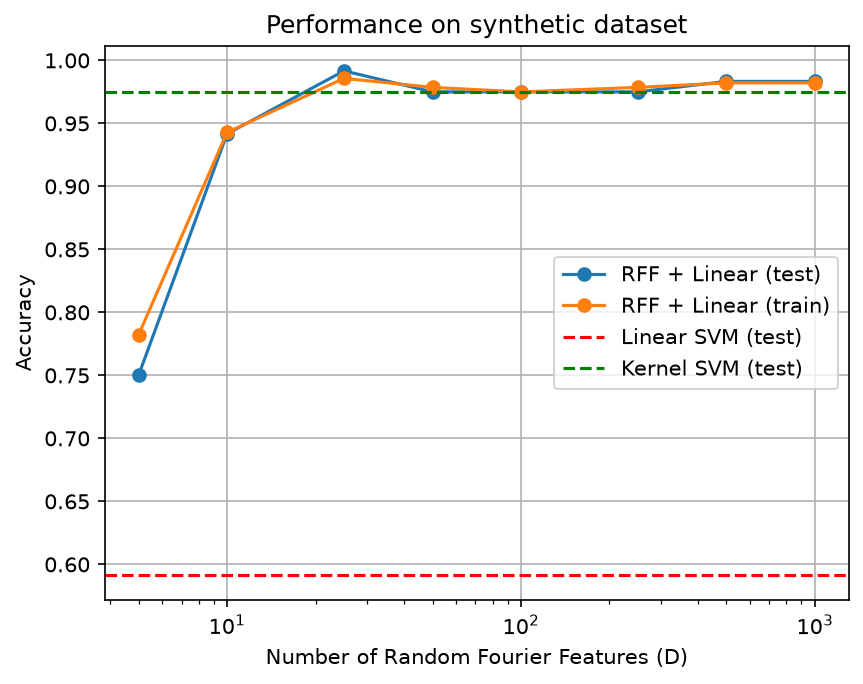
\includegraphics[width=0.75\textwidth]{../plots/synthetic_rff_comparison.png}
    \caption{Linear, kernel, and RFF comparison on the synthetic dataset.}
    \label{fig:rff_synthetic}
\end{figure}

\begin{figure}[h]
    \centering
    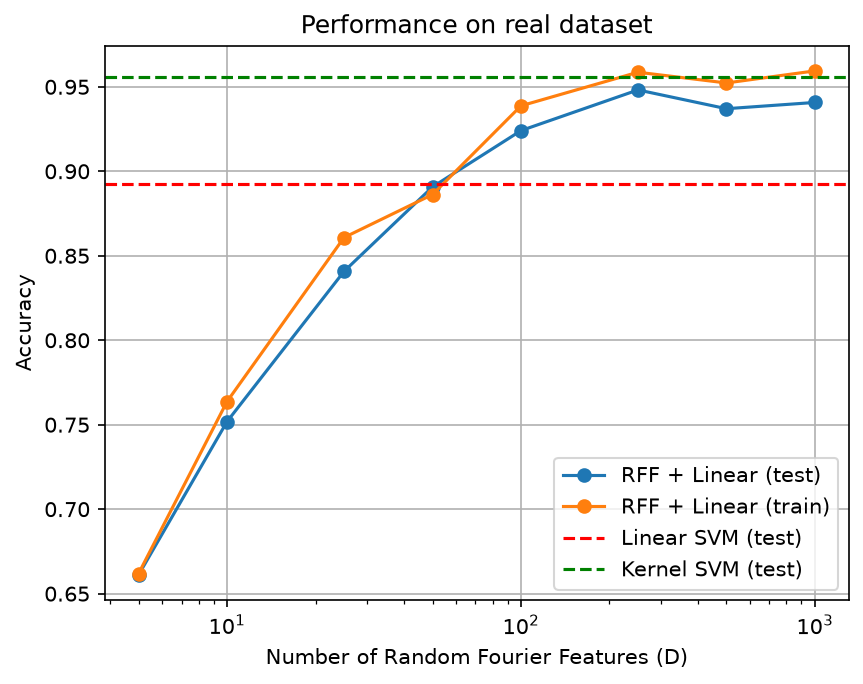
\includegraphics[width=0.75\textwidth]{../plots/real_rff_comparison.png}
    \caption{Linear, kernel, and RFF comparison on the real-world dataset.}
    \label{fig:rff_real}
\end{figure}

\FloatBarrier

\subsection{Effect of the RBF Bandwidth}
\label{ssec:gamma_ext}

Figure~\ref{fig:gamma_synthetic} and Figure~\ref{fig:gamma_real} show training and test accuracy of the kernel SVM as $\gamma$ varies, over a logarithmic grid centered on the value suggested by the median heuristic.

On the synthetic dataset, a sharp threshold behavior is observed: for $\gamma$ below approximately 0.01, test accuracy remains at exactly 50\%, indicating that the kernel is too "smoothed out" to capture any structure in the data. Past this threshold, accuracy rises sharply and stabilizes between 98\% and 99\% for the rest of the explored range, with no sign of overfitting even at the highest tested values of $\gamma$.

On the real-world dataset, the pattern is more gradual and clearly shows the "bell-shaped" trend expected from theory: test accuracy rises, peaks at 98.3\%, and then drops to 92.7\% at the highest values of $\gamma$, while training accuracy keeps rising to 100\% — a textbook case of overfitting, made possible by the dataset's higher dimensionality (64 features versus 2 in the synthetic case), which gives the kernel far more "room" to fit training-set-specific noise when the bandwidth is too narrow.

\begin{figure}[h]
    \centering
    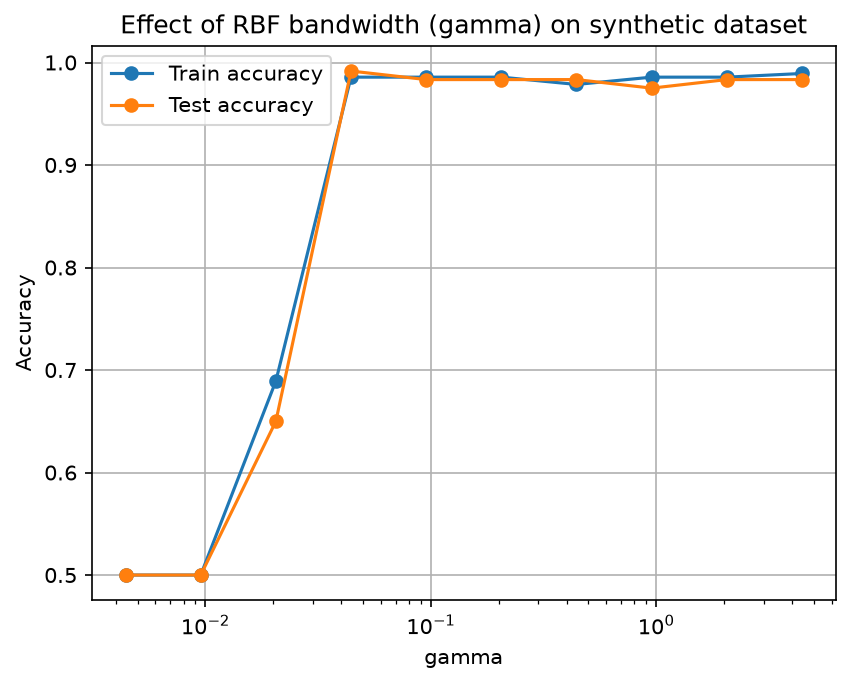
\includegraphics[width=0.75\textwidth]{../plots/synthetic_gamma_effect.png}
    \caption{Effect of the RBF bandwidth $\gamma$ on the synthetic dataset.}
    \label{fig:gamma_synthetic}
\end{figure}

\begin{figure}[h]
    \centering
    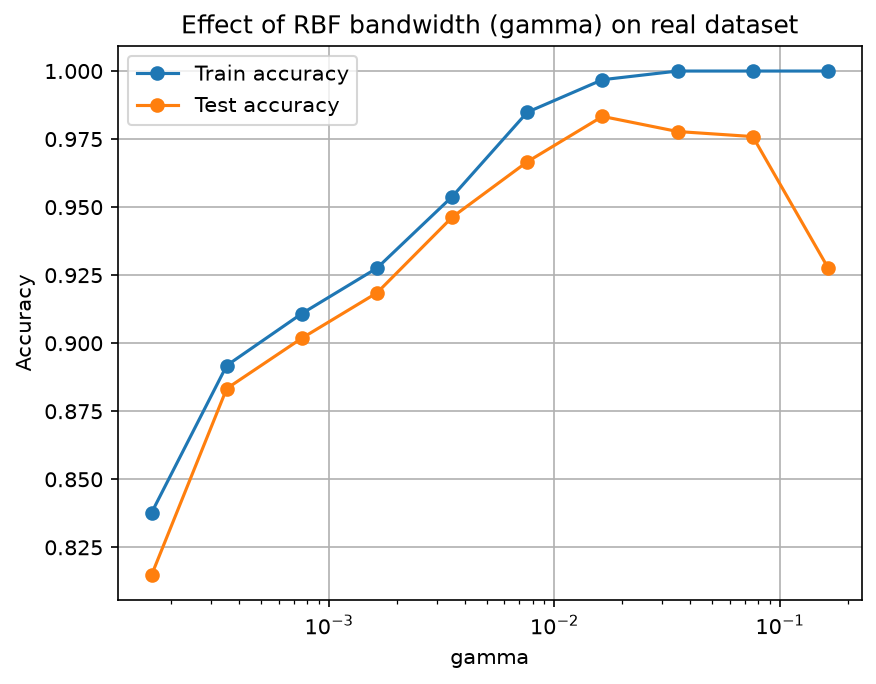
\includegraphics[width=0.75\textwidth]{../plots/real_gamma_effect.png}
    \caption{Effect of the RBF bandwidth $\gamma$ on the real-world dataset.}
    \label{fig:gamma_real}
\end{figure}

\FloatBarrier

\subsection{Random Fourier Features vs. Explicit Polynomial Feature Map}

Table~\ref{tab:poly} reports the comparison between RFF and an explicit polynomial feature map (degrees 2 and 3), in terms of accuracy and number of generated features.

On the synthetic dataset, the degree-2 polynomial feature map generates only 6 features, sufficient to reach 99.2\% test accuracy — performance comparable to RFF, but obtained with an exact (not approximated) representation and a substantially smaller number of features. Degree 3 brings no additional benefit (same 99.2\%), consistent with the fact that the XOR pattern is by construction a degree-2 interaction between the two coordinates.

On the real-world dataset, the situation reverses: the degree-2 polynomial feature map already generates 2,145 features, and degree 3 generates 47,905 — a combinatorial growth dictated by the original dimensionality of the problem (64 features), not by a free choice. Against this cost, test accuracy (97.4\% for degree 2, 97.6\% for degree 3) is comparable to that obtained by RFF with a few hundred freely-chosen features. This result concretely illustrates the practical advantage of random features over an exact but uncontrollably-dimensioned map: RFF allows explicitly choosing the trade-off between computational cost and approximation fidelity, while the polynomial feature map imposes a dimensionality dictated solely by the combinatorics of the problem.

\begin{table}[h]
\centering
\begin{tabular}{llrrr}
\toprule
Dataset & Degree & Train Acc. & Test Acc. & \# Features \\
\midrule
Synthetic & 2 & 0.9857 & 0.9917 & 6 \\
Synthetic & 3 & 0.9857 & 0.9917 & 10 \\
Real-world & 2 & 1.0000 & 0.9741 & 2145 \\
Real-world & 3 & 1.0000 & 0.9759 & 47905 \\
\bottomrule
\end{tabular}
\caption{RFF vs. explicit polynomial feature map comparison.}
\label{tab:poly}
\end{table}

\subsection{Runtime vs. Accuracy Trade-off}
\label{ssec:runtime_ext}

Figure~\ref{fig:runtime_synthetic} and Figure~\ref{fig:runtime_real} show training time (on a logarithmic scale) against test accuracy, for each model/configuration.

On the synthetic dataset, given its small size (a few hundred points), the time differences between models are modest: the exact kernel takes about 0.51 seconds versus 0.18-0.25 seconds for the RFF configurations, with the linear baseline paradoxically being slower (0.25s) despite its lower accuracy, due to the larger number of subgradient descent iterations.

On the real-world dataset, RFF's advantage becomes substantial: the exact kernel requires 15.6 seconds to train, while RFF with $D=1000$ requires only 1.3 seconds — a speed-up factor of roughly 12x — at the cost of a slightly lower accuracy (94.1\% versus 95.6\%). This result empirically confirms the practical advantage of random features as the number of training points grows: the SMO algorithm scales superlinearly with the number of samples, while the cost of RFF depends mainly on the number of features $D$, freely chosen and independent of the training set size once the transformation has been computed.

\begin{figure}[h]
    \centering
    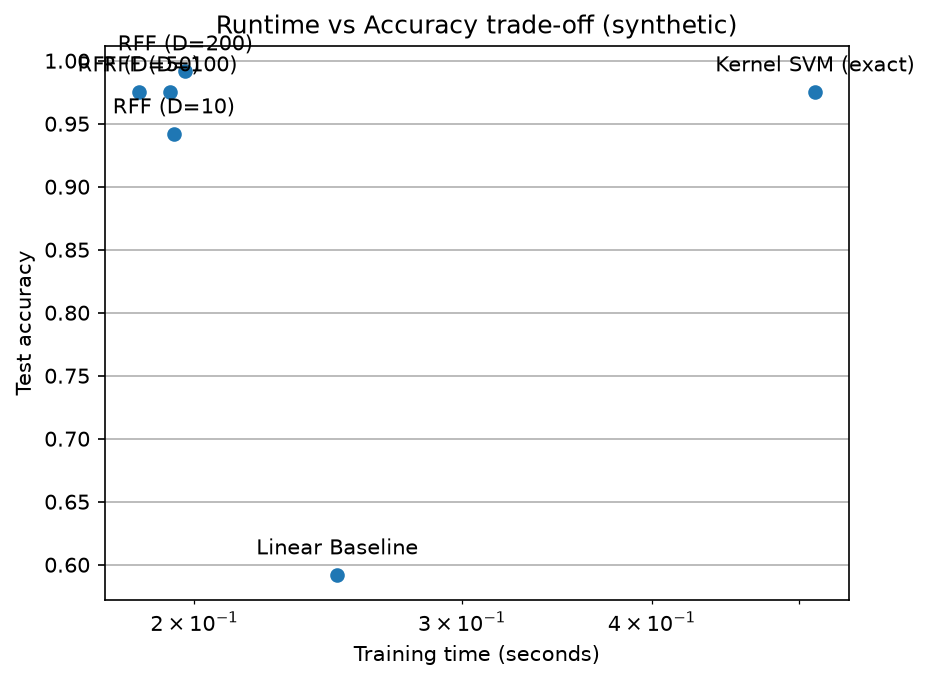
\includegraphics[width=0.75\textwidth]{../plots/synthetic_runtime_accuracy.png}
    \caption{Runtime vs. accuracy trade-off on the synthetic dataset.}
    \label{fig:runtime_synthetic}
\end{figure}

\begin{figure}[h]
    \centering
    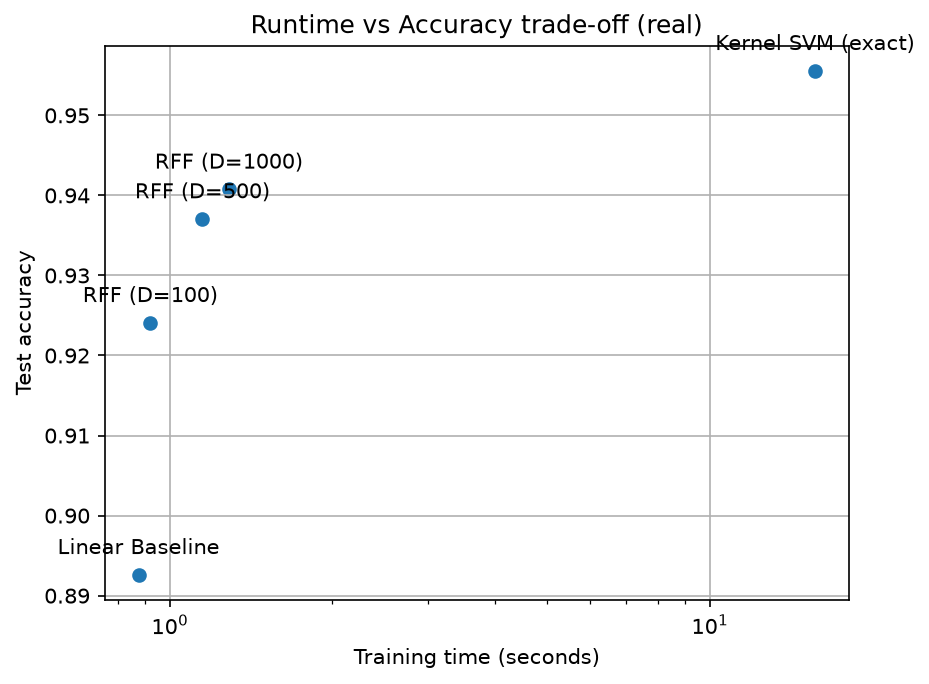
\includegraphics[width=0.75\textwidth]{../plots/real_runtime_accuracy.png}
    \caption{Runtime vs. accuracy trade-off on the real-world dataset.}
    \label{fig:runtime_real}
\end{figure}

\FloatBarrier

\section{Discussion}

The results obtained clearly confirm the theoretical expectations discussed in Section 3: a purely linear model is structurally unable to solve non-linearly separable problems (59.2\% on the XOR pattern, essentially at chance level), while both the kernel trick and Random Fourier Features recover nearly all of the gap, approaching 95-99\% accuracy on both datasets. The fact that RFF converges quickly toward the exact kernel's performance, while remaining conceptually a linear model over transformed features, empirically confirms the central thesis of the Rahimi and Recht paper: non-linearity can be "shifted" from the algorithm to the data representation, with significant computational benefits (up to 12x faster on the real-world dataset, at the cost of an accuracy loss below one percentage point).

The comparison between RFF and the explicit polynomial feature map further highlighted a relevant theoretical aspect: the dimensionality of the representation is not always a free choice. For the polynomial kernel, dimensionality is dictated by the combinatorics of the problem (growing on the order of $O(d^p)$), whereas RFF allows the trade-off between computational cost and approximation fidelity to be chosen explicitly — a non-trivial practical advantage when the original dimensionality of the data is high.

The project does, however, present some limitations worth highlighting.

First, hyperparameters other than $\gamma$ (in particular $C$ for the kernel SVM and $\lambda$ for the linear models) were fixed to reasonable values but were not systematically optimized, for example via cross-validation. It is possible that a more extensive hyperparameter search would yield somewhat different results, particularly for the kernel SVM, whose sensitivity to $C$ was not explored as thoroughly as its sensitivity to $\gamma$.

Second, the reported results derive from a single random seed per configuration. Given the stochastic nature of several components (random feature sampling, the order in which samples are visited in SMO and in subgradient descent, the train/test split), it would be advisable to repeat the experiments with multiple seeds and report the mean and standard deviation of the metrics, in order to more reliably distinguish systematic differences between models from ordinary statistical variability — a limitation particularly relevant for the close comparison between the exact kernel and RFF at high $D$, where the observed differences (e.g., 95.6\% versus 94.8\% on the real-world dataset) are of the same order of magnitude as the variability expected on a test set of a few hundred examples.

Third, the SMO implementation used performs the update loop over all training points in an unoptimized way, which limits its scalability to datasets larger than those used in this project. The training-time comparison (Section 4.4) should therefore be interpreted as indicative of the general trend (SMO scales worse than RFF as $n$ grows), rather than as an absolute measure of efficiency.

Finally, the synthetic dataset, while effective for demonstrating the linear model's limitation in a controlled way, is deliberately simple (two dimensions, four Gaussian clusters). The results obtained on it do not guarantee that the same conclusions generalize to more complex non-linear problems or to feature spaces of intermediate dimensionality, for which the real-world dataset (64 dimensions) provides only partial evidence, being itself a single case study.

\section{Conclusion}

In this project, three approaches to non-linear classification were implemented from scratch and compared: a linear SVM trained with the Pegasos algorithm, a kernel SVM with an RBF kernel trained via Sequential Minimal Optimization, and a linear model trained on top of Random Fourier Features. The comparison, carried out on a synthetic dataset designed to be non-linearly separable and on a real-world parity classification dataset of handwritten digits, clearly showed the limitations of a purely linear model and the advantage of kernel-based methods, both exact and approximated.

The main results confirm that Random Fourier Features constitute an effective approximation of the RBF kernel: as the number of random features $D$ grows, their performance quickly converges toward that of the exact kernel, at a significantly lower computational cost, especially as the size of the training set increases. The comparison with the explicit polynomial feature map further highlighted how RFF offers explicit and flexible control over the trade-off between computational cost and approximation fidelity, unlike representations whose dimensionality is dictated solely by the combinatorial structure of the problem.

Overall, the project empirically confirms the central idea of the Rahimi and Recht paper: a model's ability to capture non-linear relationships can be achieved not only through the kernel trick, but also by shifting the non-linearity into the data representation stage, with concrete practical benefits in terms of computational efficiency.

\begin{thebibliography}{9}

\bibitem{rahimi2007}
A. Rahimi and B. Recht.
\textit{Random Features for Large-Scale Kernel Machines}.
Advances in Neural Information Processing Systems (NeurIPS), 2007.

\bibitem{platt1998}
J. Platt.
\textit{Sequential Minimal Optimization: A Fast Algorithm for Training Support Vector Machines}.
Microsoft Research Technical Report MSR-TR-98-14, 1998.

\end{thebibliography}

\end{document}